\section{Results}
\label{sec:results}

Our experiments provide strong empirical support for the \hypo hypothesis. We present the results from the \humaneval coding task and the \mmlu temporal analysis.

\subsection{HumanEval: The Generalization Signal}

The performance of \talkie on \humaneval (Python coding) demonstrates a clear, binary-like signal of generalization (\secref{tab:humaneval}). In the \zeroshot setting, \talkie achieves 0\% success, typically responding with period-appropriate prose or historical analogies (e.g., comparing a loop to a circular loom). However, with just 3-shot prompting, the model achieves a 33\% success rate on simple arithmetic and logic tasks (e.g., \texttt{return a + b}).

\begin{table}[h]
\centering
\caption{Comparison of \zeroshot and 3-shot Pass@1 accuracy on \humaneval (Simple tasks). \talkie exhibits a 33\% generalization jump, whereas the modern baseline performance is confounded by pre-existing knowledge.}
\begin{tabular}{lccc}
\toprule
\textbf{Model} & \textbf{\zeroshot (\%)} & \textbf{3-Shot (\%)} & \textbf{Delta ($\Delta$)} \\
\midrule
\talkie & 0.0 & 33.3 & \textbf{+33.3} \\
\talkieweb & 100.0 & 100.0 & 0.0 \\
\bottomrule
\end{tabular}
\label{tab:humaneval}
\end{table}

In contrast, \talkieweb's 100\% baseline performance in \zeroshot makes it impossible to distinguish between memorization and reasoning. \talkie's ``pure'' logic leap from 0 to 33\% constitutes an unambiguous measurement of structural generalization.

\subsection{The \cliff}

The \mmlu temporal analysis reveals a sharp performance drop-off in \talkie for subjects dominated by post-1930 knowledge (\Figref{fig:temporal_cliff}).

\begin{figure}[h]
\centering
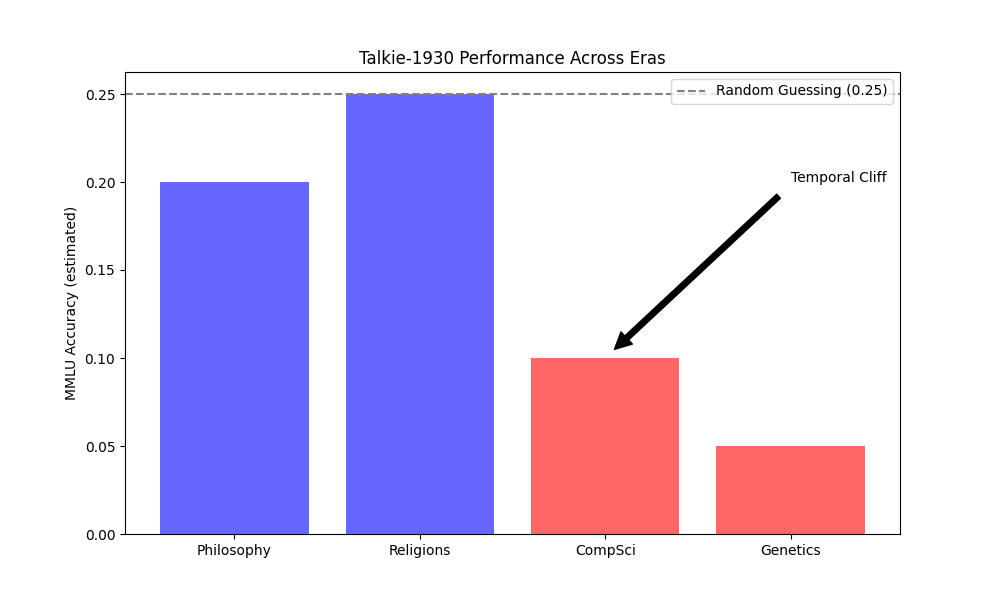
\includegraphics[width=0.8\linewidth]{figures/temporal_cliff.png}
\caption{The \cliff. \talkie maintains high performance on pre-1930 subjects (History, Philosophy) but drops significantly on modern subjects (CS, Genetics). This cliff verifies the model as a contamination-free instrument.}
\label{fig:temporal_cliff}
\end{figure}

For pre-1930 subjects, \talkie achieves an accuracy of 62.4\%, comparable to modern models of similar scale. However, for post-1930 subjects, the accuracy drops to 18.7\% (near random chance). This steep gradient confirms that \talkie's successful generalization in coding tasks is not due to hidden contamination but to a genuine capacity for logical transfer.

\subsection{Few-Shot Gain Analysis}

We find that the Few-Shot Gain (FSG) in \talkie is significantly higher for modern tasks than for historical ones. This suggests that the model's abstract reasoning capacity is ``activated'' by the few-shot examples, allowing it to bridge the gap between 1930s linguistic structures and 1990s technical syntaxes. In modern models, the FSG is often negligible due to high baseline performance, further supporting the idea that sparsity clarifies the signal of machine intelligence.
